% TODO:
% * Fix plotting of optimal portfolio.
% * Make it solid. Understand and check it.

\documentclass[a4paper]{article}

\usepackage{graphicx}
\usepackage{float}
\usepackage{amsmath}
\usepackage[utf8]{inputenc}
\usepackage[english]{babel}
\usepackage[bookmarks=true]{hyperref}
\usepackage{color}
\usepackage{listings}

\usepackage[
    type={CC},
    modifier={by-nc-sa},
    version={3.0},
]{doclicense}

\usepackage{xcolor}
% New colors defined below.
\definecolor{codegreen}{rgb}{0,0.6,0}
\definecolor{codegray}{rgb}{0.5,0.5,0.5}
\definecolor{codepurple}{rgb}{0.58,0,0.82}
\definecolor{backcolour}{rgb}{0.95,0.95,0.92}

%Code listing style named "mystyle"
\lstdefinestyle{mystyle}{
%  backgroundcolor=\color{backcolour},
  commentstyle=\color{codegreen},
  keywordstyle=\color{magenta},
  numberstyle=\tiny\color{codegray},
  stringstyle=\color{codepurple},
  basicstyle=\ttfamily\footnotesize,
  breakatwhitespace=false,
  breaklines=true,
  keepspaces=true,
  numbers=left,
  numbersep=5pt,
  showspaces=false,
  showstringspaces=false,
  showtabs=false,
  tabsize=2
}

%"mystyle" code listing set
\lstset{style=mystyle}

\def\documenttitle{Frans' Savings Plan}

\title{\documenttitle}
\date{\today}
\author{Frans Englich \\
        \href{mailto:fenglich@fastmail.fm}{fenglich@fastmail.fm}}

\hypersetup{
    pdfsubject = {\documenttitle},
    pdftitle = {\documenttitle}
}

\begin{document}

\maketitle

My idea is it would be wise to save for pension or large investment such as an apartment. My interest in this, beyond the end result, is limited: I have no intension to spend time on fundamental analysis or follow developments on a regular basis. However, I do write this document, and I intend to do a modern portfolio theory (MPT) analysis of the portfolio. I have in interest to sleep well, without worrying about this.

Individual stocks are, as far as I can tell, hence irrelevant because I won't manage it, rebalance, and so forth. Therefore I think it makes sense to look at passive indices and active management.

The computations contains no strategic decisions, they are a procedural, technical matter. The interesting questions is what assets to choose, and that is the hard part, not calculating the portfolio weights.

\section{Details}

This is the broad picture:

\begin{itemize}
\item "Long" horizon. Easily 5-10 years
\item Generally offensive/"high" risk investment
\item Bank of choice is Avanza in Sweden
\item Other banks of mine are Nordea in Sweden and Norway. A student's economy, only savings accounts
\item Account type for the investments: Investeringssparkonto (ISK)
\item Start amount: 10 000 SEK
\item Monthly investment: 500 SEK.
\end{itemize}

\section{Investment Objects}

\begin{table}[H]
    \label{table_assets}
    \begin{center}
    \begin{tabular}{ |l|l|l|l| }
        \hline
        Name & Short name & Type & Total Fee (for funds) \\
        \hline
        \href{https://www.avanza.se/aktier/om-aktien.html/338588/creades-a}{Creades A} & CRED A & Investment company & - \\
        \href{https://www.avanza.se/aktier/om-aktien.html/5245/industrivarden-c}{Industrivärden C} & INDU C & Investment company & - \\
        \href{https://www.avanza.se/fonder/om-fonden.html/929/seb-europafond-smabolag}{SEB Europafond Småbolag} & - & Fund & 2.01\% \\
        \href{https://www.avanza.se/fonder/om-fonden.html/70331/ms-invf-us-growth-a-usd}{MS INVF US Growth A USD} & - & Fund & 1.80\% \\
        \hline
    \end{tabular}
    \end{center}
    \caption{Selected assets for the portfolio.}
\end{table}

In short, according to my very shallow approach to this, I say it achieves diversification across USA, Europe and Sweden, and is high return/risk. Therefore it matches my objectives.

\section{A Modern Portfolio Theory Analysis}

The objective is to maximise the portfolio's Sharpe ratio and acquire informational key figures. That is, the tangency portfolio is of interest. Therefore I will compute the portfolio's:

\begin{itemize}
    \item Mean-variance efficient asset weights
    \item Efficient frontier
    \item Expected return
    \item Standard deviation
    \item Sharpe ratio.
% VaR?
\end{itemize}

\subsection{Mean-variance Efficient Frontier}

Mathematically, the problem is:

\begin{equation*}
    \max_{w} w'\mu
\end{equation*}

\(w\) is a \(N\times1\) vector of asset weights, where \(N\) is the number of assets. $\mu$ is a \(N\times1\) vector of expected returns. The solution can be found in the mean-variance efficient frontier, which is:

\begin{equation*}
    \bar{u}_p = \frac{A}{C} + \frac{1}{C} \sqrt{(C\sigma^2_p - 1)(BC - A^2)},
\end{equation*}

where

\begin{align*}
    A &= \mu'\Sigma^{-1}\iota  \\
    B &= \mu'\Sigma^{-1}\mu    \\
    C &= \iota\Sigma^{-1}\iota \\
\end{align*}

$\Sigma$ is an \(N\times N\) variance-covariance matrix of returns, $\iota$ an \(N\times 1\) vector of ones.

The mean-variance frontier for the portfolio is plotted in figure \ref{figure_mv_frontier}.

\begin{figure}[H]
    \centering
    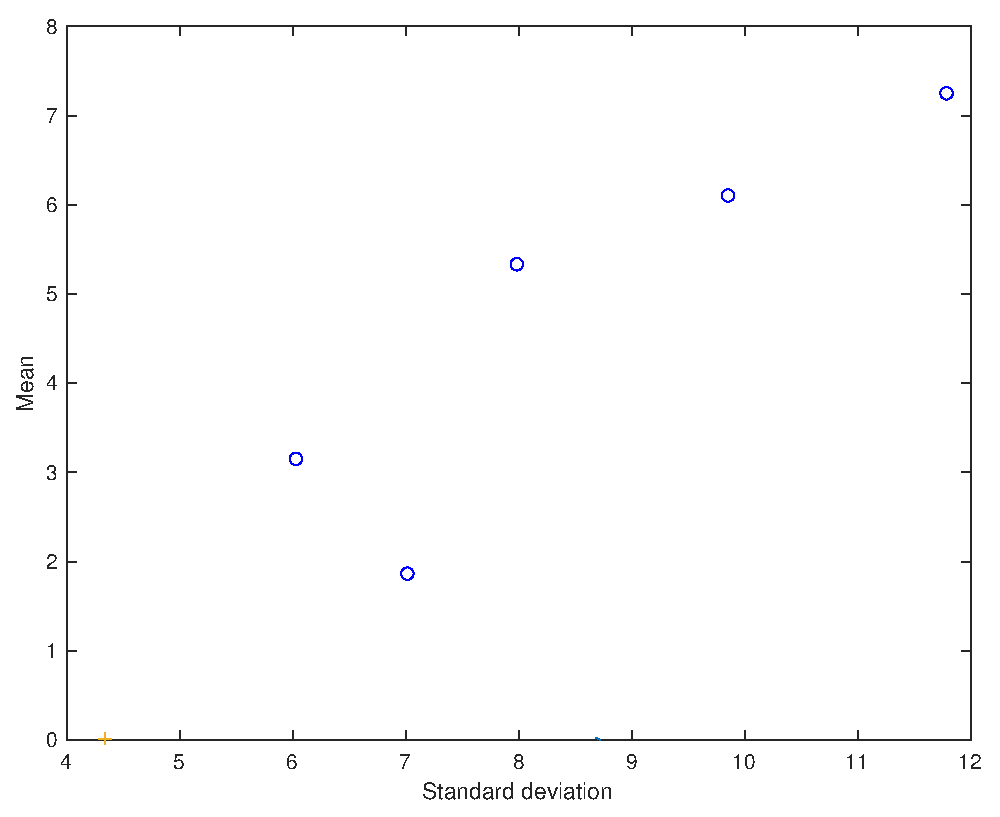
\includegraphics[width=0.7\textwidth, keepaspectratio]{figures/mv_frontier.eps}
    \caption{Mean-variance frontier of portfolio.}
    \label{figure_mv_frontier}
\end{figure}

\section{Optimal Weights}

The optimal weights of the assets in the portfolio are found in table \ref{table_optimal_weights}. The optimal weights may involve shorting, but due to the bank not allowing this, the optimisation has been constrained to not include shorting.

\begin{table}[H]
    \begin{center}
    \begin{tabular}{ |l|l|l| }
        \hline
        Asset Name & Weighting & Weighting (\%) \\
        \hline

        1 & 0.238727 & 24 \\
2 & 0.213544 & 21 \\
3 & 0.328114 & 33 \\
4 & 0.130888 & 13 \\
5 & 0.088728 & 9 \\


        \hline
    \end{tabular}
    \caption{Optimal weights.}
    \label{table_optimal_weights}
    \end{center}
\end{table}



\section{Remaining Questions}

\appendix

\section{Code}

\lstinputlisting[language=Matlab, caption=Matlab code]{frontier.m}

\section{License}

\doclicenseThis

\end{document}
